\documentclass[twoside]{book}

% Packages required by doxygen
\usepackage{fixltx2e}
\usepackage{calc}
\usepackage{doxygen}
\usepackage[export]{adjustbox} % also loads graphicx
\usepackage{graphicx}
\usepackage[utf8]{inputenc}
\usepackage{makeidx}
\usepackage{multicol}
\usepackage{multirow}
\PassOptionsToPackage{warn}{textcomp}
\usepackage{textcomp}
\usepackage[nointegrals]{wasysym}
\usepackage[table]{xcolor}

% NLS support packages
\usepackage[french]{babel}

% Font selection
\usepackage[T1]{fontenc}
\usepackage[scaled=.90]{helvet}
\usepackage{courier}
\usepackage{amssymb}
\usepackage{sectsty}
\renewcommand{\familydefault}{\sfdefault}
\allsectionsfont{%
  \fontseries{bc}\selectfont%
  \color{darkgray}%
}
\renewcommand{\DoxyLabelFont}{%
  \fontseries{bc}\selectfont%
  \color{darkgray}%
}
\newcommand{\+}{\discretionary{\mbox{\scriptsize$\hookleftarrow$}}{}{}}

% Page & text layout
\usepackage{geometry}
\geometry{%
  a4paper,%
  top=2.5cm,%
  bottom=2.5cm,%
  left=2.5cm,%
  right=2.5cm%
}
\tolerance=750
\hfuzz=15pt
\hbadness=750
\setlength{\emergencystretch}{15pt}
\setlength{\parindent}{0cm}
\setlength{\parskip}{3ex plus 2ex minus 2ex}
\makeatletter
\renewcommand{\paragraph}{%
  \@startsection{paragraph}{4}{0ex}{-1.0ex}{1.0ex}{%
    \normalfont\normalsize\bfseries\SS@parafont%
  }%
}
\renewcommand{\subparagraph}{%
  \@startsection{subparagraph}{5}{0ex}{-1.0ex}{1.0ex}{%
    \normalfont\normalsize\bfseries\SS@subparafont%
  }%
}
\makeatother

% Headers & footers
\usepackage{fancyhdr}
\pagestyle{fancyplain}
\fancyhead[LE]{\fancyplain{}{\bfseries\thepage}}
\fancyhead[CE]{\fancyplain{}{}}
\fancyhead[RE]{\fancyplain{}{\bfseries\leftmark}}
\fancyhead[LO]{\fancyplain{}{\bfseries\rightmark}}
\fancyhead[CO]{\fancyplain{}{}}
\fancyhead[RO]{\fancyplain{}{\bfseries\thepage}}
\fancyfoot[LE]{\fancyplain{}{}}
\fancyfoot[CE]{\fancyplain{}{}}
\fancyfoot[RE]{\fancyplain{}{\bfseries\scriptsize Généré par Doxygen }}
\fancyfoot[LO]{\fancyplain{}{\bfseries\scriptsize Généré par Doxygen }}
\fancyfoot[CO]{\fancyplain{}{}}
\fancyfoot[RO]{\fancyplain{}{}}
\renewcommand{\footrulewidth}{0.4pt}
\renewcommand{\chaptermark}[1]{%
  \markboth{#1}{}%
}
\renewcommand{\sectionmark}[1]{%
  \markright{\thesection\ #1}%
}

% Indices & bibliography
\usepackage{natbib}
\usepackage[titles]{tocloft}
\setcounter{tocdepth}{3}
\setcounter{secnumdepth}{5}
\makeindex

% Hyperlinks (required, but should be loaded last)
\usepackage{ifpdf}
\ifpdf
  \usepackage[pdftex,pagebackref=true]{hyperref}
\else
  \usepackage[ps2pdf,pagebackref=true]{hyperref}
\fi
\hypersetup{%
  colorlinks=true,%
  linkcolor=blue,%
  citecolor=blue,%
  unicode%
}

% Custom commands
\newcommand{\clearemptydoublepage}{%
  \newpage{\pagestyle{empty}\cleardoublepage}%
}

\usepackage{caption}
\captionsetup{labelsep=space,justification=centering,font={bf},singlelinecheck=off,skip=4pt,position=top}

%===== C O N T E N T S =====

\begin{document}

% Titlepage & ToC
\hypersetup{pageanchor=false,
             bookmarksnumbered=true,
             pdfencoding=unicode
            }
\pagenumbering{alph}
\begin{titlepage}
\vspace*{7cm}
\begin{center}%
{\Large GoL \\[1ex]\large 2.\+0.\+0 }\\
\vspace*{1cm}
{\large Généré par Doxygen 1.8.13}\\
\end{center}
\end{titlepage}
\clearemptydoublepage
\pagenumbering{roman}
\tableofcontents
\clearemptydoublepage
\pagenumbering{arabic}
\hypersetup{pageanchor=true}

%--- Begin generated contents ---
\chapter{Index des classes}
\section{Liste des classes}
Liste des classes, structures, unions et interfaces avec une brève description \+:\begin{DoxyCompactList}
\item\contentsline{section}{\hyperlink{structgrille}{grille} \\*Structure grille\+: le type principal du jeu, qui contient informations sur le tableau de cellules }{\pageref{structgrille}}{}
\end{DoxyCompactList}

\chapter{Index des fichiers}
\section{Liste des fichiers}
Liste de tous les fichiers documentés avec une brève description \+:\begin{DoxyCompactList}
\item\contentsline{section}{\hyperlink{grille_8c}{grille.\+c} }{\pageref{grille_8c}}{}
\item\contentsline{section}{\hyperlink{grille_8h}{grille.\+h} \\*Fichier entête du code source \hyperlink{grille_8c}{grille.\+c} }{\pageref{grille_8h}}{}
\item\contentsline{section}{\hyperlink{io_8c}{io.\+c} }{\pageref{io_8c}}{}
\item\contentsline{section}{\hyperlink{io_8h}{io.\+h} \\*Fichier entête du code source \hyperlink{io_8c}{io.\+c} }{\pageref{io_8h}}{}
\item\contentsline{section}{\hyperlink{jeu_8c}{jeu.\+c} }{\pageref{jeu_8c}}{}
\item\contentsline{section}{\hyperlink{jeu_8h}{jeu.\+h} \\*Fichier entête du code source \hyperlink{jeu_8c}{jeu.\+c} }{\pageref{jeu_8h}}{}
\item\contentsline{section}{\hyperlink{main_8c}{main.\+c} }{\pageref{main_8c}}{}
\end{DoxyCompactList}

\chapter{Documentation des classes}
\hypertarget{structgrille}{}\section{Référence de la structure grille}
\label{structgrille}\index{grille@{grille}}


structure grille\+: le type principal du jeu, qui contient informations sur le tableau de cellules  




{\ttfamily \#include $<$grille.\+h$>$}

\subsection*{Attributs publics}
\begin{DoxyCompactItemize}
\item 
int \hyperlink{structgrille_a0b4da1e205825df205b0c004d105d62a}{nbl}
\item 
int \hyperlink{structgrille_a48d6706d41bee6fff9200d872b8b0cd0}{nbc}
\item 
int $\ast$$\ast$ \hyperlink{structgrille_a428cf0c0297ce04e0206ba0067ac3b42}{cellules}
\end{DoxyCompactItemize}


\subsection{Description détaillée}
structure grille\+: le type principal du jeu, qui contient informations sur le tableau de cellules 

\subsection{Documentation des données membres}
\mbox{\Hypertarget{structgrille_a428cf0c0297ce04e0206ba0067ac3b42}\label{structgrille_a428cf0c0297ce04e0206ba0067ac3b42}} 
\index{grille@{grille}!cellules@{cellules}}
\index{cellules@{cellules}!grille@{grille}}
\subsubsection{\texorpdfstring{cellules}{cellules}}
{\footnotesize\ttfamily int$\ast$$\ast$ grille\+::cellules}

tableau de tableau de cellules \mbox{\Hypertarget{structgrille_a48d6706d41bee6fff9200d872b8b0cd0}\label{structgrille_a48d6706d41bee6fff9200d872b8b0cd0}} 
\index{grille@{grille}!nbc@{nbc}}
\index{nbc@{nbc}!grille@{grille}}
\subsubsection{\texorpdfstring{nbc}{nbc}}
{\footnotesize\ttfamily int grille\+::nbc}

nombre de colonnes \mbox{\Hypertarget{structgrille_a0b4da1e205825df205b0c004d105d62a}\label{structgrille_a0b4da1e205825df205b0c004d105d62a}} 
\index{grille@{grille}!nbl@{nbl}}
\index{nbl@{nbl}!grille@{grille}}
\subsubsection{\texorpdfstring{nbl}{nbl}}
{\footnotesize\ttfamily int grille\+::nbl}

nombre de lignes 

La documentation de cette structure a été générée à partir du fichier suivant \+:\begin{DoxyCompactItemize}
\item 
\hyperlink{grille_8h}{grille.\+h}\end{DoxyCompactItemize}

\chapter{Documentation des fichiers}
\hypertarget{grille_8c}{}\section{Référence du fichier src/grille.c}
\label{grille_8c}\index{src/grille.\+c@{src/grille.\+c}}
{\ttfamily \#include $<$assert.\+h$>$}\newline
{\ttfamily \#include $<$errno.\+h$>$}\newline
{\ttfamily \#include $<$stdio.\+h$>$}\newline
{\ttfamily \#include $<$stdlib.\+h$>$}\newline
{\ttfamily \#include $<$string.\+h$>$}\newline
{\ttfamily \#include $<$cairo.\+h$>$}\newline
{\ttfamily \#include $<$cairo-\/xlib.\+h$>$}\newline
{\ttfamily \#include $<$X11/\+Xlib.\+h$>$}\newline
{\ttfamily \#include \char`\"{}grille.\+h\char`\"{}}\newline
Graphe des dépendances par inclusion de grille.\+c\+:
\nopagebreak
\begin{figure}[H]
\begin{center}
\leavevmode
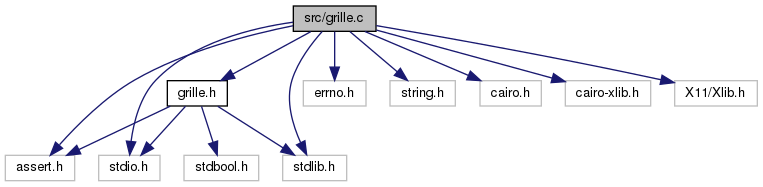
\includegraphics[width=350pt]{grille_8c__incl}
\end{center}
\end{figure}
\subsection*{Fonctions}
\begin{DoxyCompactItemize}
\item 
void \hyperlink{grille_8c_ae621f51c60aa4fafaa0c9f6c9b5a4036}{alloue\+\_\+grille} (int l, int c, \hyperlink{structgrille}{grille} $\ast$g)
\begin{DoxyCompactList}\small\item\em alloue une grille de taille l$\ast$c, et initialise toutes les cellules a mortes \end{DoxyCompactList}\item 
void \hyperlink{grille_8c_a7074b2b15576e9d2b3cd15c3a1dc7012}{libere\+\_\+grille} (\hyperlink{structgrille}{grille} $\ast$g)
\begin{DoxyCompactList}\small\item\em permet de liberer la memoire allouee pour les cellules \end{DoxyCompactList}\item 
void \hyperlink{grille_8c_ac247d94af4c53fe64b28236f0a507bf0}{init\+\_\+grille\+\_\+from\+\_\+file} (char const $\ast$const filename, \hyperlink{structgrille}{grille} $\ast$g)
\begin{DoxyCompactList}\small\item\em init\+\_\+grille\+\_\+from\+\_\+file alloue et initalise la grille g a partir d\textquotesingle{}un fichier \end{DoxyCompactList}\item 
void \hyperlink{grille_8c_a4562474d3f481fa7da7133925c37b99b}{copie\+\_\+grille} (\hyperlink{structgrille}{grille} $\ast$\hyperlink{grille_8c_a83c67db95a5b42df92b41f8fa9982502}{gs}, \hyperlink{structgrille}{grille} $\ast$gd)
\begin{DoxyCompactList}\small\item\em copie\+\_\+grille recopie gs dans gd \end{DoxyCompactList}\item 
bool \hyperlink{grille_8c_af12c2156faaf6b18dd0ade10fbe629de}{meme\+\_\+grille} (\hyperlink{structgrille}{grille} $\ast$\hyperlink{grille_8c_a83c67db95a5b42df92b41f8fa9982502}{gs}, \hyperlink{structgrille}{grille} $\ast$gd)
\begin{DoxyCompactList}\small\item\em meme\+\_\+grille test si gs et gd soit meme \end{DoxyCompactList}\item 
\mbox{\Hypertarget{grille_8c_a092a39783960ddbee5acc32c9b6864b5}\label{grille_8c_a092a39783960ddbee5acc32c9b6864b5}} 
int {\bfseries est\+\_\+vivante} (int i, int j, \hyperlink{structgrille}{grille} g)
\item 
\mbox{\Hypertarget{grille_8c_a3e49f2869c8721e998df4096674b950e}\label{grille_8c_a3e49f2869c8721e998df4096674b950e}} 
int {\bfseries est\+\_\+nonvia} (int i, int j, \hyperlink{structgrille}{grille} g)
\item 
\mbox{\Hypertarget{grille_8c_ae0cbadbe963314bacd54c1a1ea511da7}\label{grille_8c_ae0cbadbe963314bacd54c1a1ea511da7}} 
void {\bfseries set\+\_\+vivante} (int i, int j, \hyperlink{structgrille}{grille} g)
\item 
\mbox{\Hypertarget{grille_8c_a3d327664dfff09d6528dce52687f0a15}\label{grille_8c_a3d327664dfff09d6528dce52687f0a15}} 
void {\bfseries set\+\_\+nonvia} (int i, int j, \hyperlink{structgrille}{grille} g)
\item 
\mbox{\Hypertarget{grille_8c_a3c8e6e08e82824278fdf45a4a05dc85a}\label{grille_8c_a3c8e6e08e82824278fdf45a4a05dc85a}} 
void {\bfseries set\+\_\+morte} (int i, int j, \hyperlink{structgrille}{grille} g)
\end{DoxyCompactItemize}
\subsection*{Variables}
\begin{DoxyCompactItemize}
\item 
\mbox{\Hypertarget{grille_8c_a83c67db95a5b42df92b41f8fa9982502}\label{grille_8c_a83c67db95a5b42df92b41f8fa9982502}} 
\hyperlink{structgrille}{grille} \hyperlink{grille_8c_a83c67db95a5b42df92b41f8fa9982502}{gs}
\begin{DoxyCompactList}\small\item\em On definie global gs,gg ici. \end{DoxyCompactList}\item 
\mbox{\Hypertarget{grille_8c_ac5c92d5caaf5856349597ac5352eaf56}\label{grille_8c_ac5c92d5caaf5856349597ac5352eaf56}} 
\hyperlink{structgrille}{grille} {\bfseries gg}
\end{DoxyCompactItemize}


\subsection{Description détaillée}
\begin{DoxyAuthor}{Auteur}
D\+AI Yuquan 
\end{DoxyAuthor}


\subsection{Documentation des fonctions}
\mbox{\Hypertarget{grille_8c_ae621f51c60aa4fafaa0c9f6c9b5a4036}\label{grille_8c_ae621f51c60aa4fafaa0c9f6c9b5a4036}} 
\index{grille.\+c@{grille.\+c}!alloue\+\_\+grille@{alloue\+\_\+grille}}
\index{alloue\+\_\+grille@{alloue\+\_\+grille}!grille.\+c@{grille.\+c}}
\subsubsection{\texorpdfstring{alloue\+\_\+grille()}{alloue\_grille()}}
{\footnotesize\ttfamily void alloue\+\_\+grille (\begin{DoxyParamCaption}\item[{int}]{l,  }\item[{int}]{c,  }\item[{\hyperlink{structgrille}{grille} $\ast$}]{g }\end{DoxyParamCaption})}



alloue une grille de taille l$\ast$c, et initialise toutes les cellules a mortes 


\begin{DoxyParams}{Paramètres}
{\em l} & nombre de lignes \\
\hline
{\em c} & nombre de colonnes \\
\hline
{\em g} & grille \\
\hline
\end{DoxyParams}
\mbox{\Hypertarget{grille_8c_a4562474d3f481fa7da7133925c37b99b}\label{grille_8c_a4562474d3f481fa7da7133925c37b99b}} 
\index{grille.\+c@{grille.\+c}!copie\+\_\+grille@{copie\+\_\+grille}}
\index{copie\+\_\+grille@{copie\+\_\+grille}!grille.\+c@{grille.\+c}}
\subsubsection{\texorpdfstring{copie\+\_\+grille()}{copie\_grille()}}
{\footnotesize\ttfamily void copie\+\_\+grille (\begin{DoxyParamCaption}\item[{\hyperlink{structgrille}{grille} $\ast$}]{gs,  }\item[{\hyperlink{structgrille}{grille} $\ast$}]{gd }\end{DoxyParamCaption})}



copie\+\_\+grille recopie gs dans gd 


\begin{DoxyParams}{Paramètres}
{\em gs} & grille \\
\hline
{\em gd} & grille \\
\hline
\end{DoxyParams}
\mbox{\Hypertarget{grille_8c_ac247d94af4c53fe64b28236f0a507bf0}\label{grille_8c_ac247d94af4c53fe64b28236f0a507bf0}} 
\index{grille.\+c@{grille.\+c}!init\+\_\+grille\+\_\+from\+\_\+file@{init\+\_\+grille\+\_\+from\+\_\+file}}
\index{init\+\_\+grille\+\_\+from\+\_\+file@{init\+\_\+grille\+\_\+from\+\_\+file}!grille.\+c@{grille.\+c}}
\subsubsection{\texorpdfstring{init\+\_\+grille\+\_\+from\+\_\+file()}{init\_grille\_from\_file()}}
{\footnotesize\ttfamily void init\+\_\+grille\+\_\+from\+\_\+file (\begin{DoxyParamCaption}\item[{char const $\ast$const}]{filename,  }\item[{\hyperlink{structgrille}{grille} $\ast$}]{g }\end{DoxyParamCaption})}



init\+\_\+grille\+\_\+from\+\_\+file alloue et initalise la grille g a partir d\textquotesingle{}un fichier 


\begin{DoxyParams}{Paramètres}
{\em filename} & nom du fichier a ouvrir \\
\hline
{\em g} & grille \\
\hline
\end{DoxyParams}
\mbox{\Hypertarget{grille_8c_a7074b2b15576e9d2b3cd15c3a1dc7012}\label{grille_8c_a7074b2b15576e9d2b3cd15c3a1dc7012}} 
\index{grille.\+c@{grille.\+c}!libere\+\_\+grille@{libere\+\_\+grille}}
\index{libere\+\_\+grille@{libere\+\_\+grille}!grille.\+c@{grille.\+c}}
\subsubsection{\texorpdfstring{libere\+\_\+grille()}{libere\_grille()}}
{\footnotesize\ttfamily void libere\+\_\+grille (\begin{DoxyParamCaption}\item[{\hyperlink{structgrille}{grille} $\ast$}]{g }\end{DoxyParamCaption})}



permet de liberer la memoire allouee pour les cellules 


\begin{DoxyParams}{Paramètres}
{\em g} & grille \\
\hline
\end{DoxyParams}
\mbox{\Hypertarget{grille_8c_af12c2156faaf6b18dd0ade10fbe629de}\label{grille_8c_af12c2156faaf6b18dd0ade10fbe629de}} 
\index{grille.\+c@{grille.\+c}!meme\+\_\+grille@{meme\+\_\+grille}}
\index{meme\+\_\+grille@{meme\+\_\+grille}!grille.\+c@{grille.\+c}}
\subsubsection{\texorpdfstring{meme\+\_\+grille()}{meme\_grille()}}
{\footnotesize\ttfamily bool meme\+\_\+grille (\begin{DoxyParamCaption}\item[{\hyperlink{structgrille}{grille} $\ast$}]{gs,  }\item[{\hyperlink{structgrille}{grille} $\ast$}]{gd }\end{DoxyParamCaption})}



meme\+\_\+grille test si gs et gd soit meme 


\begin{DoxyParams}{Paramètres}
{\em gs} & grille \\
\hline
{\em gd} & grille \\
\hline
\end{DoxyParams}
\begin{DoxyReturn}{Renvoie}
test true ou false 
\end{DoxyReturn}

\hypertarget{grille_8h}{}\section{Référence du fichier grille.\+h}
\label{grille_8h}\index{grille.\+h@{grille.\+h}}


Fichier entête du code source \hyperlink{grille_8c}{grille.\+c}.  


{\ttfamily \#include $<$stdlib.\+h$>$}\newline
{\ttfamily \#include $<$stdio.\+h$>$}\newline
{\ttfamily \#include $<$assert.\+h$>$}\newline
Graphe des dépendances par inclusion de grille.\+h\+:
% FIG 0
Ce graphe montre quels fichiers incluent directement ou indirectement ce fichier \+:
% FIG 1
\subsection*{Classes}
\begin{DoxyCompactItemize}
\item 
struct \hyperlink{structgrille}{grille}
\begin{DoxyCompactList}\small\item\em structure grille\+: le type principal du jeu, qui contient informations sur le tableau de cellules \end{DoxyCompactList}\end{DoxyCompactItemize}
\subsection*{Fonctions}
\begin{DoxyCompactItemize}
\item 
void \hyperlink{grille_8h_ae621f51c60aa4fafaa0c9f6c9b5a4036}{alloue\+\_\+grille} (int l, int c, \hyperlink{structgrille}{grille} $\ast$g)
\begin{DoxyCompactList}\small\item\em alloue une grille de taille l$\ast$c, et initialise toutes les cellules a mortes \end{DoxyCompactList}\item 
void \hyperlink{grille_8h_a7074b2b15576e9d2b3cd15c3a1dc7012}{libere\+\_\+grille} (\hyperlink{structgrille}{grille} $\ast$g)
\begin{DoxyCompactList}\small\item\em permet de liberer la memoire allouee pour les cellules \end{DoxyCompactList}\item 
void \hyperlink{grille_8h_adf5501cc0bbad28f5ffc561d92197e4e}{init\+\_\+grille\+\_\+from\+\_\+file} (char $\ast$filename, \hyperlink{structgrille}{grille} $\ast$g)
\begin{DoxyCompactList}\small\item\em init\+\_\+grille\+\_\+from\+\_\+file alloue et initalise la grille g a partir d\textquotesingle{}un fichier \end{DoxyCompactList}\item 
\mbox{\Hypertarget{grille_8h_ae0cbadbe963314bacd54c1a1ea511da7}\label{grille_8h_ae0cbadbe963314bacd54c1a1ea511da7}} 
void {\bfseries set\+\_\+vivante} (int i, int j, \hyperlink{structgrille}{grille} g)
\item 
\mbox{\Hypertarget{grille_8h_a3c8e6e08e82824278fdf45a4a05dc85a}\label{grille_8h_a3c8e6e08e82824278fdf45a4a05dc85a}} 
void {\bfseries set\+\_\+morte} (int i, int j, \hyperlink{structgrille}{grille} g)
\item 
\mbox{\Hypertarget{grille_8h_a092a39783960ddbee5acc32c9b6864b5}\label{grille_8h_a092a39783960ddbee5acc32c9b6864b5}} 
int {\bfseries est\+\_\+vivante} (int i, int j, \hyperlink{structgrille}{grille} g)
\item 
void \hyperlink{grille_8h_a63b3ae16c86b568f6aa8f9ce84128b1e}{copie\+\_\+grille} (\hyperlink{structgrille}{grille} gs, \hyperlink{structgrille}{grille} gd)
\begin{DoxyCompactList}\small\item\em copie\+\_\+grille recopie gs dans gd \end{DoxyCompactList}\end{DoxyCompactItemize}


\subsection{Description détaillée}
Fichier entête du code source \hyperlink{grille_8c}{grille.\+c}. 

\begin{DoxyAuthor}{Auteur}
D\+AI Yuquan 
\end{DoxyAuthor}


\subsection{Documentation des fonctions}
\mbox{\Hypertarget{grille_8h_ae621f51c60aa4fafaa0c9f6c9b5a4036}\label{grille_8h_ae621f51c60aa4fafaa0c9f6c9b5a4036}} 
\index{grille.\+h@{grille.\+h}!alloue\+\_\+grille@{alloue\+\_\+grille}}
\index{alloue\+\_\+grille@{alloue\+\_\+grille}!grille.\+h@{grille.\+h}}
\subsubsection{\texorpdfstring{alloue\+\_\+grille()}{alloue\_grille()}}
{\footnotesize\ttfamily void alloue\+\_\+grille (\begin{DoxyParamCaption}\item[{int}]{l,  }\item[{int}]{c,  }\item[{\hyperlink{structgrille}{grille} $\ast$}]{g }\end{DoxyParamCaption})}



alloue une grille de taille l$\ast$c, et initialise toutes les cellules a mortes 


\begin{DoxyParams}{Paramètres}
{\em l} & nombre de lignes \\
\hline
{\em c} & nombre de colonnes \\
\hline
{\em g} & grille \\
\hline
\end{DoxyParams}
\mbox{\Hypertarget{grille_8h_a63b3ae16c86b568f6aa8f9ce84128b1e}\label{grille_8h_a63b3ae16c86b568f6aa8f9ce84128b1e}} 
\index{grille.\+h@{grille.\+h}!copie\+\_\+grille@{copie\+\_\+grille}}
\index{copie\+\_\+grille@{copie\+\_\+grille}!grille.\+h@{grille.\+h}}
\subsubsection{\texorpdfstring{copie\+\_\+grille()}{copie\_grille()}}
{\footnotesize\ttfamily void copie\+\_\+grille (\begin{DoxyParamCaption}\item[{\hyperlink{structgrille}{grille}}]{gs,  }\item[{\hyperlink{structgrille}{grille}}]{gd }\end{DoxyParamCaption})}



copie\+\_\+grille recopie gs dans gd 


\begin{DoxyParams}{Paramètres}
{\em gs} & grille \\
\hline
{\em gd} & grille \\
\hline
\end{DoxyParams}
\mbox{\Hypertarget{grille_8h_adf5501cc0bbad28f5ffc561d92197e4e}\label{grille_8h_adf5501cc0bbad28f5ffc561d92197e4e}} 
\index{grille.\+h@{grille.\+h}!init\+\_\+grille\+\_\+from\+\_\+file@{init\+\_\+grille\+\_\+from\+\_\+file}}
\index{init\+\_\+grille\+\_\+from\+\_\+file@{init\+\_\+grille\+\_\+from\+\_\+file}!grille.\+h@{grille.\+h}}
\subsubsection{\texorpdfstring{init\+\_\+grille\+\_\+from\+\_\+file()}{init\_grille\_from\_file()}}
{\footnotesize\ttfamily void init\+\_\+grille\+\_\+from\+\_\+file (\begin{DoxyParamCaption}\item[{char $\ast$}]{filename,  }\item[{\hyperlink{structgrille}{grille} $\ast$}]{g }\end{DoxyParamCaption})}



init\+\_\+grille\+\_\+from\+\_\+file alloue et initalise la grille g a partir d\textquotesingle{}un fichier 


\begin{DoxyParams}{Paramètres}
{\em filename} & nom du fichier a ouvrir \\
\hline
{\em g} & grille \\
\hline
\end{DoxyParams}
\mbox{\Hypertarget{grille_8h_a7074b2b15576e9d2b3cd15c3a1dc7012}\label{grille_8h_a7074b2b15576e9d2b3cd15c3a1dc7012}} 
\index{grille.\+h@{grille.\+h}!libere\+\_\+grille@{libere\+\_\+grille}}
\index{libere\+\_\+grille@{libere\+\_\+grille}!grille.\+h@{grille.\+h}}
\subsubsection{\texorpdfstring{libere\+\_\+grille()}{libere\_grille()}}
{\footnotesize\ttfamily void libere\+\_\+grille (\begin{DoxyParamCaption}\item[{\hyperlink{structgrille}{grille} $\ast$}]{g }\end{DoxyParamCaption})}



permet de liberer la memoire allouee pour les cellules 


\begin{DoxyParams}{Paramètres}
{\em g} & grille \\
\hline
\end{DoxyParams}

\hypertarget{io_8c}{}\section{Référence du fichier src/io.c}
\label{io_8c}\index{src/io.\+c@{src/io.\+c}}
{\ttfamily \#include $<$cairo.\+h$>$}\newline
{\ttfamily \#include $<$cairo-\/xlib.\+h$>$}\newline
{\ttfamily \#include $<$X11/\+Xlib.\+h$>$}\newline
{\ttfamily \#include $<$X11/keysymdef.\+h$>$}\newline
{\ttfamily \#include $<$string.\+h$>$}\newline
{\ttfamily \#include $<$stdlib.\+h$>$}\newline
{\ttfamily \#include $<$X11/\+X\+K\+Blib.\+h$>$}\newline
{\ttfamily \#include \char`\"{}io.\+h\char`\"{}}\newline
{\ttfamily \#include \char`\"{}grille.\+h\char`\"{}}\newline
Graphe des dépendances par inclusion de io.\+c\+:
\nopagebreak
\begin{figure}[H]
\begin{center}
\leavevmode
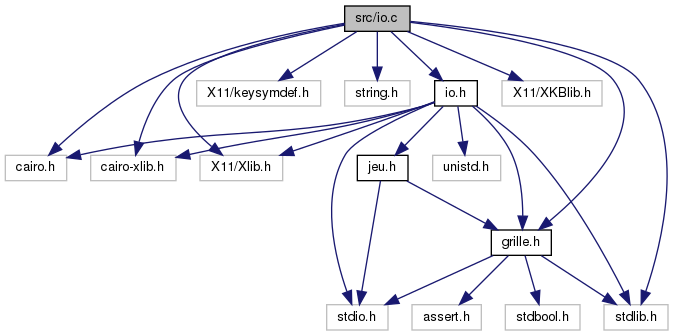
\includegraphics[width=350pt]{io_8c__incl}
\end{center}
\end{figure}
\subsection*{Fonctions}
\begin{DoxyCompactItemize}
\item 
\mbox{\Hypertarget{io_8c_a7488d6302931e47bb5516246528ba930}\label{io_8c_a7488d6302931e47bb5516246528ba930}} 
void \hyperlink{io_8c_a7488d6302931e47bb5516246528ba930}{init\+\_\+surface} ()
\begin{DoxyCompactList}\small\item\em initialise l\textquotesingle{}ecran graphique \end{DoxyCompactList}\item 
void \hyperlink{io_8c_a09f1f9ebde686da54bf440c149be532d}{affiche\+\_\+cairo\+\_\+text} (int x, int y, char $\ast$text)
\begin{DoxyCompactList}\small\item\em affiche un string sur l\textquotesingle{}ecran graphique \end{DoxyCompactList}\item 
void \hyperlink{io_8c_a17bf4c475aa40bc4fc9bff937dbcd02b}{dessine\+\_\+cairo\+\_\+ligne} (int x1, int y1, int x2, int y2)
\begin{DoxyCompactList}\small\item\em desine une ligne sur l\textquotesingle{}ecran graphique \end{DoxyCompactList}\item 
void \hyperlink{io_8c_a1f465e0c96abf80471766204b50b071c}{affiche\+\_\+cellule} (int x, int y, int val, int vieillissement)
\begin{DoxyCompactList}\small\item\em affiche une cellule de la grille \end{DoxyCompactList}\item 
void \hyperlink{io_8c_a0f5ec4fd3b3993b83114188fb065bedd}{affiche\+\_\+ligne} (int x, int y, int $\ast$ligne, int vieillissement)
\begin{DoxyCompactList}\small\item\em affiche une ligne de la grille sur l\textquotesingle{}ecran graphique \end{DoxyCompactList}\item 
void \hyperlink{io_8c_a3fbc5daf7726bc8805bf43deebd992df}{affiche\+\_\+grille} (\hyperlink{structgrille}{grille} g, char $\ast$modec, char $\ast$modev, int vieillissement)
\begin{DoxyCompactList}\small\item\em affiche la grille \end{DoxyCompactList}\item 
void \hyperlink{io_8c_a312d20304b2ce3d21b8c9b6f1c7e7495}{affiche\+\_\+osc} (\hyperlink{structgrille}{grille} $\ast$g, \hyperlink{structgrille}{grille} $\ast$gc)
\begin{DoxyCompactList}\small\item\em test si les cellules sont oscillantes \end{DoxyCompactList}\item 
void \hyperlink{io_8c_a88493b3c55828670e47150a95ed7db5b}{debut\+\_\+jeu} (\hyperlink{structgrille}{grille} $\ast$g, \hyperlink{structgrille}{grille} $\ast$gc)
\begin{DoxyCompactList}\small\item\em debute le jeu \end{DoxyCompactList}\end{DoxyCompactItemize}
\subsection*{Variables}
\begin{DoxyCompactItemize}
\item 
\mbox{\Hypertarget{io_8c_a5eb3d60e246c25f6b3f30ef9d6aa26d2}\label{io_8c_a5eb3d60e246c25f6b3f30ef9d6aa26d2}} 
Display $\ast$ \hyperlink{io_8c_a5eb3d60e246c25f6b3f30ef9d6aa26d2}{D\+PY}
\begin{DoxyCompactList}\small\item\em l\textquotesingle{}ecran graphique \end{DoxyCompactList}\item 
\mbox{\Hypertarget{io_8c_aa627f2d78166d6a48da70b2b57e1b2e6}\label{io_8c_aa627f2d78166d6a48da70b2b57e1b2e6}} 
cairo\+\_\+surface\+\_\+t $\ast$ \hyperlink{io_8c_aa627f2d78166d6a48da70b2b57e1b2e6}{CS}
\begin{DoxyCompactList}\small\item\em liason avec l\textquotesingle{}ecran graphique par cairo \end{DoxyCompactList}\item 
\mbox{\Hypertarget{io_8c_af2ea217fbc26cf40f7f878835be462a8}\label{io_8c_af2ea217fbc26cf40f7f878835be462a8}} 
cairo\+\_\+t $\ast$ \hyperlink{io_8c_af2ea217fbc26cf40f7f878835be462a8}{CR}
\begin{DoxyCompactList}\small\item\em la masque avec laquelle on affiche tout \end{DoxyCompactList}\item 
\mbox{\Hypertarget{io_8c_a3fb05c7269d3ff36c95d9166d2fb5e83}\label{io_8c_a3fb05c7269d3ff36c95d9166d2fb5e83}} 
cairo\+\_\+surface\+\_\+t $\ast$ {\bfseries image\+\_\+B}
\item 
\mbox{\Hypertarget{io_8c_a8f24c221e2ba6c65cb329a8c41a242d9}\label{io_8c_a8f24c221e2ba6c65cb329a8c41a242d9}} 
cairo\+\_\+t $\ast$ {\bfseries image\+\_\+dc\+\_\+B}
\item 
\mbox{\Hypertarget{io_8c_aef8c3edbbd56b8f2052628fb7dc69660}\label{io_8c_aef8c3edbbd56b8f2052628fb7dc69660}} 
cairo\+\_\+surface\+\_\+t $\ast$ {\bfseries oscplate}
\item 
\mbox{\Hypertarget{io_8c_a088620e913482b370648d77005b5cca7}\label{io_8c_a088620e913482b370648d77005b5cca7}} 
cairo\+\_\+t $\ast$ {\bfseries oscplate\+\_\+dc}
\item 
\mbox{\Hypertarget{io_8c_a0bb2c810f4d06f86aaa032da354a92e2}\label{io_8c_a0bb2c810f4d06f86aaa032da354a92e2}} 
int \hyperlink{io_8c_a0bb2c810f4d06f86aaa032da354a92e2}{temps\+\_\+evolution} =0
\begin{DoxyCompactList}\small\item\em on garde le temps d\textquotesingle{}evolution ici \end{DoxyCompactList}\end{DoxyCompactItemize}


\subsection{Description détaillée}
\begin{DoxyAuthor}{Auteur}
D\+AI Yuquan 
\end{DoxyAuthor}


\subsection{Documentation des fonctions}
\mbox{\Hypertarget{io_8c_a09f1f9ebde686da54bf440c149be532d}\label{io_8c_a09f1f9ebde686da54bf440c149be532d}} 
\index{io.\+c@{io.\+c}!affiche\+\_\+cairo\+\_\+text@{affiche\+\_\+cairo\+\_\+text}}
\index{affiche\+\_\+cairo\+\_\+text@{affiche\+\_\+cairo\+\_\+text}!io.\+c@{io.\+c}}
\subsubsection{\texorpdfstring{affiche\+\_\+cairo\+\_\+text()}{affiche\_cairo\_text()}}
{\footnotesize\ttfamily void affiche\+\_\+cairo\+\_\+text (\begin{DoxyParamCaption}\item[{int}]{x,  }\item[{int}]{y,  }\item[{char $\ast$}]{text }\end{DoxyParamCaption})}



affiche un string sur l\textquotesingle{}ecran graphique 


\begin{DoxyParams}{Paramètres}
{\em x} & coordone x \\
\hline
{\em y} & coordone y \\
\hline
{\em text} & le string qui sera afiche \\
\hline
\end{DoxyParams}
\mbox{\Hypertarget{io_8c_a1f465e0c96abf80471766204b50b071c}\label{io_8c_a1f465e0c96abf80471766204b50b071c}} 
\index{io.\+c@{io.\+c}!affiche\+\_\+cellule@{affiche\+\_\+cellule}}
\index{affiche\+\_\+cellule@{affiche\+\_\+cellule}!io.\+c@{io.\+c}}
\subsubsection{\texorpdfstring{affiche\+\_\+cellule()}{affiche\_cellule()}}
{\footnotesize\ttfamily void affiche\+\_\+cellule (\begin{DoxyParamCaption}\item[{int}]{x,  }\item[{int}]{y,  }\item[{int}]{val,  }\item[{int}]{vieillissement }\end{DoxyParamCaption})}



affiche une cellule de la grille 


\begin{DoxyParams}{Paramètres}
{\em x} & coordonne x du point de debut de l\textquotesingle{}affichage \\
\hline
{\em y} & coordonne y du point de debut de l\textquotesingle{}affichage \\
\hline
{\em val} & valeur de la cellule \\
\hline
{\em vieillissement} & si true, on montre l\textquotesingle{}ages des cellules et non si false \\
\hline
\end{DoxyParams}
\mbox{\Hypertarget{io_8c_a3fbc5daf7726bc8805bf43deebd992df}\label{io_8c_a3fbc5daf7726bc8805bf43deebd992df}} 
\index{io.\+c@{io.\+c}!affiche\+\_\+grille@{affiche\+\_\+grille}}
\index{affiche\+\_\+grille@{affiche\+\_\+grille}!io.\+c@{io.\+c}}
\subsubsection{\texorpdfstring{affiche\+\_\+grille()}{affiche\_grille()}}
{\footnotesize\ttfamily void affiche\+\_\+grille (\begin{DoxyParamCaption}\item[{\hyperlink{structgrille}{grille}}]{g,  }\item[{char $\ast$}]{modec,  }\item[{char $\ast$}]{modev,  }\item[{int}]{vieillissement }\end{DoxyParamCaption})}



affiche la grille 


\begin{DoxyParams}{Paramètres}
{\em g} & grille \\
\hline
{\em modec} & text pour circuler \\
\hline
{\em modev} & text pour vieillissement \\
\hline
{\em vieillissement} & si true, on montre l\textquotesingle{}ages des cellules et non si false \\
\hline
\end{DoxyParams}
\mbox{\Hypertarget{io_8c_a0f5ec4fd3b3993b83114188fb065bedd}\label{io_8c_a0f5ec4fd3b3993b83114188fb065bedd}} 
\index{io.\+c@{io.\+c}!affiche\+\_\+ligne@{affiche\+\_\+ligne}}
\index{affiche\+\_\+ligne@{affiche\+\_\+ligne}!io.\+c@{io.\+c}}
\subsubsection{\texorpdfstring{affiche\+\_\+ligne()}{affiche\_ligne()}}
{\footnotesize\ttfamily void affiche\+\_\+ligne (\begin{DoxyParamCaption}\item[{int}]{x,  }\item[{int}]{y,  }\item[{int $\ast$}]{ligne,  }\item[{int}]{vieillissement }\end{DoxyParamCaption})}



affiche une ligne de la grille sur l\textquotesingle{}ecran graphique 


\begin{DoxyParams}{Paramètres}
{\em x} & nombre d\textquotesingle{}elements de la ligne \\
\hline
{\em y} & nombre de la ligne \\
\hline
{\em ligne} & une ligne de la grille \\
\hline
{\em vieillissement} & si true, on montre l\textquotesingle{}ages des cellules et non si false \\
\hline
\end{DoxyParams}
\mbox{\Hypertarget{io_8c_a312d20304b2ce3d21b8c9b6f1c7e7495}\label{io_8c_a312d20304b2ce3d21b8c9b6f1c7e7495}} 
\index{io.\+c@{io.\+c}!affiche\+\_\+osc@{affiche\+\_\+osc}}
\index{affiche\+\_\+osc@{affiche\+\_\+osc}!io.\+c@{io.\+c}}
\subsubsection{\texorpdfstring{affiche\+\_\+osc()}{affiche\_osc()}}
{\footnotesize\ttfamily void affiche\+\_\+osc (\begin{DoxyParamCaption}\item[{\hyperlink{structgrille}{grille} $\ast$}]{g,  }\item[{\hyperlink{structgrille}{grille} $\ast$}]{gc }\end{DoxyParamCaption})}



test si les cellules sont oscillantes 


\begin{DoxyParams}{Paramètres}
{\em g} & grille \\
\hline
{\em gc} & grille pour evoluer \\
\hline
\end{DoxyParams}
\mbox{\Hypertarget{io_8c_a88493b3c55828670e47150a95ed7db5b}\label{io_8c_a88493b3c55828670e47150a95ed7db5b}} 
\index{io.\+c@{io.\+c}!debut\+\_\+jeu@{debut\+\_\+jeu}}
\index{debut\+\_\+jeu@{debut\+\_\+jeu}!io.\+c@{io.\+c}}
\subsubsection{\texorpdfstring{debut\+\_\+jeu()}{debut\_jeu()}}
{\footnotesize\ttfamily void debut\+\_\+jeu (\begin{DoxyParamCaption}\item[{\hyperlink{structgrille}{grille} $\ast$}]{g,  }\item[{\hyperlink{structgrille}{grille} $\ast$}]{gc }\end{DoxyParamCaption})}



debute le jeu 


\begin{DoxyParams}{Paramètres}
{\em g} & grille \\
\hline
{\em gc} & grille \\
\hline
\end{DoxyParams}
\mbox{\Hypertarget{io_8c_a17bf4c475aa40bc4fc9bff937dbcd02b}\label{io_8c_a17bf4c475aa40bc4fc9bff937dbcd02b}} 
\index{io.\+c@{io.\+c}!dessine\+\_\+cairo\+\_\+ligne@{dessine\+\_\+cairo\+\_\+ligne}}
\index{dessine\+\_\+cairo\+\_\+ligne@{dessine\+\_\+cairo\+\_\+ligne}!io.\+c@{io.\+c}}
\subsubsection{\texorpdfstring{dessine\+\_\+cairo\+\_\+ligne()}{dessine\_cairo\_ligne()}}
{\footnotesize\ttfamily void dessine\+\_\+cairo\+\_\+ligne (\begin{DoxyParamCaption}\item[{int}]{x1,  }\item[{int}]{y1,  }\item[{int}]{x2,  }\item[{int}]{y2 }\end{DoxyParamCaption})}



desine une ligne sur l\textquotesingle{}ecran graphique 


\begin{DoxyParams}{Paramètres}
{\em x1} & coordonne x du premier point \\
\hline
{\em y1} & coordonne y du premier point \\
\hline
{\em x2} & coordonne x du second point \\
\hline
{\em y2} & coordonne x du second point \\
\hline
\end{DoxyParams}

\hypertarget{io_8h}{}\section{Référence du fichier include/io.h}
\label{io_8h}\index{include/io.\+h@{include/io.\+h}}


Fichier entête du code source \hyperlink{io_8c}{io.\+c}.  


{\ttfamily \#include $<$stdio.\+h$>$}\newline
{\ttfamily \#include $<$stdlib.\+h$>$}\newline
{\ttfamily \#include $<$unistd.\+h$>$}\newline
{\ttfamily \#include $<$cairo.\+h$>$}\newline
{\ttfamily \#include $<$cairo-\/xlib.\+h$>$}\newline
{\ttfamily \#include $<$X11/\+Xlib.\+h$>$}\newline
{\ttfamily \#include \char`\"{}grille.\+h\char`\"{}}\newline
{\ttfamily \#include \char`\"{}jeu.\+h\char`\"{}}\newline
Graphe des dépendances par inclusion de io.\+h\+:
\nopagebreak
\begin{figure}[H]
\begin{center}
\leavevmode
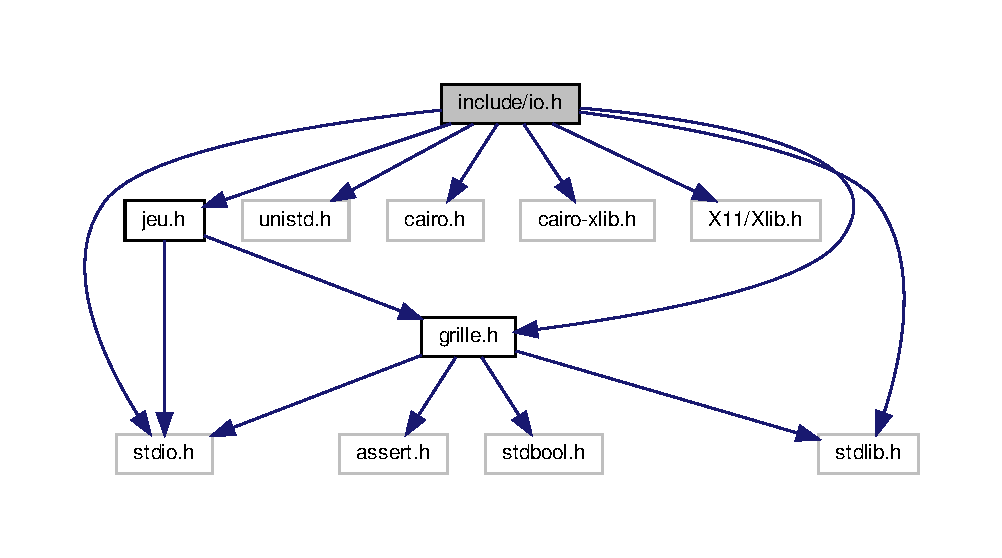
\includegraphics[width=350pt]{io_8h__incl}
\end{center}
\end{figure}
Ce graphe montre quels fichiers incluent directement ou indirectement ce fichier \+:
\nopagebreak
\begin{figure}[H]
\begin{center}
\leavevmode
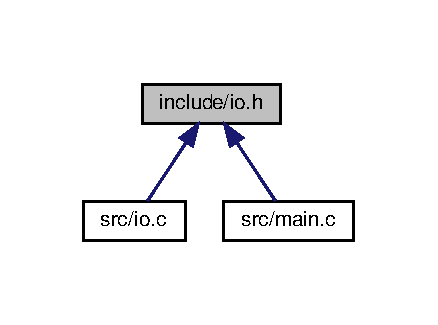
\includegraphics[width=210pt]{io_8h__dep__incl}
\end{center}
\end{figure}
\subsection*{Macros}
\begin{DoxyCompactItemize}
\item 
\#define \hyperlink{io_8h_a3d6d12a6ee0d7d77f3f180ed1b2a1e22}{S\+I\+Z\+EX}~1000
\item 
\#define \hyperlink{io_8h_a7e1991fcd344daa8c9e423cfd3481a8c}{S\+I\+Z\+EY}~800
\end{DoxyCompactItemize}
\subsection*{Fonctions}
\begin{DoxyCompactItemize}
\item 
\mbox{\Hypertarget{io_8h_a7488d6302931e47bb5516246528ba930}\label{io_8h_a7488d6302931e47bb5516246528ba930}} 
void \hyperlink{io_8h_a7488d6302931e47bb5516246528ba930}{init\+\_\+surface} ()
\begin{DoxyCompactList}\small\item\em initialise l\textquotesingle{}ecran graphique \end{DoxyCompactList}\item 
void \hyperlink{io_8h_a0f5ec4fd3b3993b83114188fb065bedd}{affiche\+\_\+ligne} (int x, int y, int $\ast$ligne, int vieillissement)
\begin{DoxyCompactList}\small\item\em affiche une ligne de la grille sur l\textquotesingle{}ecran graphique \end{DoxyCompactList}\item 
void \hyperlink{io_8h_a3fbc5daf7726bc8805bf43deebd992df}{affiche\+\_\+grille} (\hyperlink{structgrille}{grille} g, char $\ast$modec, char $\ast$modev, int vieillissement)
\begin{DoxyCompactList}\small\item\em affiche la grille \end{DoxyCompactList}\item 
void \hyperlink{io_8h_a09f1f9ebde686da54bf440c149be532d}{affiche\+\_\+cairo\+\_\+text} (int x, int y, char $\ast$text)
\begin{DoxyCompactList}\small\item\em affiche un string sur l\textquotesingle{}ecran graphique \end{DoxyCompactList}\item 
void \hyperlink{io_8h_a17bf4c475aa40bc4fc9bff937dbcd02b}{dessine\+\_\+cairo\+\_\+ligne} (int x1, int y1, int x2, int y2)
\begin{DoxyCompactList}\small\item\em desine une ligne sur l\textquotesingle{}ecran graphique \end{DoxyCompactList}\item 
void \hyperlink{io_8h_a1f465e0c96abf80471766204b50b071c}{affiche\+\_\+cellule} (int x, int y, int val, int vieillissement)
\begin{DoxyCompactList}\small\item\em affiche une cellule de la grille \end{DoxyCompactList}\item 
void \hyperlink{io_8h_a312d20304b2ce3d21b8c9b6f1c7e7495}{affiche\+\_\+osc} (\hyperlink{structgrille}{grille} $\ast$g, \hyperlink{structgrille}{grille} $\ast$gc)
\begin{DoxyCompactList}\small\item\em test si les cellules sont oscillantes \end{DoxyCompactList}\item 
void \hyperlink{io_8h_a88493b3c55828670e47150a95ed7db5b}{debut\+\_\+jeu} (\hyperlink{structgrille}{grille} $\ast$g, \hyperlink{structgrille}{grille} $\ast$gc)
\begin{DoxyCompactList}\small\item\em debute le jeu \end{DoxyCompactList}\end{DoxyCompactItemize}
\subsection*{Variables}
\begin{DoxyCompactItemize}
\item 
\mbox{\Hypertarget{io_8h_a5eb3d60e246c25f6b3f30ef9d6aa26d2}\label{io_8h_a5eb3d60e246c25f6b3f30ef9d6aa26d2}} 
Display $\ast$ \hyperlink{io_8h_a5eb3d60e246c25f6b3f30ef9d6aa26d2}{D\+PY}
\begin{DoxyCompactList}\small\item\em l\textquotesingle{}ecran graphique \end{DoxyCompactList}\item 
\mbox{\Hypertarget{io_8h_aa627f2d78166d6a48da70b2b57e1b2e6}\label{io_8h_aa627f2d78166d6a48da70b2b57e1b2e6}} 
cairo\+\_\+surface\+\_\+t $\ast$ \hyperlink{io_8h_aa627f2d78166d6a48da70b2b57e1b2e6}{CS}
\begin{DoxyCompactList}\small\item\em liason avec l\textquotesingle{}ecran graphique par cairo \end{DoxyCompactList}\item 
\mbox{\Hypertarget{io_8h_af2ea217fbc26cf40f7f878835be462a8}\label{io_8h_af2ea217fbc26cf40f7f878835be462a8}} 
cairo\+\_\+t $\ast$ \hyperlink{io_8h_af2ea217fbc26cf40f7f878835be462a8}{CR}
\begin{DoxyCompactList}\small\item\em la masque avec laquelle on affiche tout \end{DoxyCompactList}\item 
\mbox{\Hypertarget{io_8h_a0bb2c810f4d06f86aaa032da354a92e2}\label{io_8h_a0bb2c810f4d06f86aaa032da354a92e2}} 
int \hyperlink{io_8h_a0bb2c810f4d06f86aaa032da354a92e2}{temps\+\_\+evolution}
\begin{DoxyCompactList}\small\item\em on garde le temps d\textquotesingle{}evolution ici \end{DoxyCompactList}\end{DoxyCompactItemize}


\subsection{Description détaillée}
Fichier entête du code source \hyperlink{io_8c}{io.\+c}. 

\begin{DoxyAuthor}{Auteur}
D\+AI Yuquan 
\end{DoxyAuthor}


\subsection{Documentation des macros}
\mbox{\Hypertarget{io_8h_a3d6d12a6ee0d7d77f3f180ed1b2a1e22}\label{io_8h_a3d6d12a6ee0d7d77f3f180ed1b2a1e22}} 
\index{io.\+h@{io.\+h}!S\+I\+Z\+EX@{S\+I\+Z\+EX}}
\index{S\+I\+Z\+EX@{S\+I\+Z\+EX}!io.\+h@{io.\+h}}
\subsubsection{\texorpdfstring{S\+I\+Z\+EX}{SIZEX}}
{\footnotesize\ttfamily \#define S\+I\+Z\+EX~1000}

largeur de l\textquotesingle{}ecran graphique \mbox{\Hypertarget{io_8h_a7e1991fcd344daa8c9e423cfd3481a8c}\label{io_8h_a7e1991fcd344daa8c9e423cfd3481a8c}} 
\index{io.\+h@{io.\+h}!S\+I\+Z\+EY@{S\+I\+Z\+EY}}
\index{S\+I\+Z\+EY@{S\+I\+Z\+EY}!io.\+h@{io.\+h}}
\subsubsection{\texorpdfstring{S\+I\+Z\+EY}{SIZEY}}
{\footnotesize\ttfamily \#define S\+I\+Z\+EY~800}

longeur de l\textquotesingle{}ecran graphique 

\subsection{Documentation des fonctions}
\mbox{\Hypertarget{io_8h_a09f1f9ebde686da54bf440c149be532d}\label{io_8h_a09f1f9ebde686da54bf440c149be532d}} 
\index{io.\+h@{io.\+h}!affiche\+\_\+cairo\+\_\+text@{affiche\+\_\+cairo\+\_\+text}}
\index{affiche\+\_\+cairo\+\_\+text@{affiche\+\_\+cairo\+\_\+text}!io.\+h@{io.\+h}}
\subsubsection{\texorpdfstring{affiche\+\_\+cairo\+\_\+text()}{affiche\_cairo\_text()}}
{\footnotesize\ttfamily void affiche\+\_\+cairo\+\_\+text (\begin{DoxyParamCaption}\item[{int}]{x,  }\item[{int}]{y,  }\item[{char $\ast$}]{text }\end{DoxyParamCaption})}



affiche un string sur l\textquotesingle{}ecran graphique 


\begin{DoxyParams}{Paramètres}
{\em x} & coordone x \\
\hline
{\em y} & coordone y \\
\hline
{\em text} & le string qui sera afiche \\
\hline
\end{DoxyParams}
\mbox{\Hypertarget{io_8h_a1f465e0c96abf80471766204b50b071c}\label{io_8h_a1f465e0c96abf80471766204b50b071c}} 
\index{io.\+h@{io.\+h}!affiche\+\_\+cellule@{affiche\+\_\+cellule}}
\index{affiche\+\_\+cellule@{affiche\+\_\+cellule}!io.\+h@{io.\+h}}
\subsubsection{\texorpdfstring{affiche\+\_\+cellule()}{affiche\_cellule()}}
{\footnotesize\ttfamily void affiche\+\_\+cellule (\begin{DoxyParamCaption}\item[{int}]{x,  }\item[{int}]{y,  }\item[{int}]{val,  }\item[{int}]{vieillissement }\end{DoxyParamCaption})}



affiche une cellule de la grille 


\begin{DoxyParams}{Paramètres}
{\em x} & coordonne x du point de debut de l\textquotesingle{}affichage \\
\hline
{\em y} & coordonne y du point de debut de l\textquotesingle{}affichage \\
\hline
{\em val} & valeur de la cellule \\
\hline
{\em vieillissement} & si true, on montre l\textquotesingle{}ages des cellules et non si false \\
\hline
\end{DoxyParams}
\mbox{\Hypertarget{io_8h_a3fbc5daf7726bc8805bf43deebd992df}\label{io_8h_a3fbc5daf7726bc8805bf43deebd992df}} 
\index{io.\+h@{io.\+h}!affiche\+\_\+grille@{affiche\+\_\+grille}}
\index{affiche\+\_\+grille@{affiche\+\_\+grille}!io.\+h@{io.\+h}}
\subsubsection{\texorpdfstring{affiche\+\_\+grille()}{affiche\_grille()}}
{\footnotesize\ttfamily void affiche\+\_\+grille (\begin{DoxyParamCaption}\item[{\hyperlink{structgrille}{grille}}]{g,  }\item[{char $\ast$}]{modec,  }\item[{char $\ast$}]{modev,  }\item[{int}]{vieillissement }\end{DoxyParamCaption})}



affiche la grille 


\begin{DoxyParams}{Paramètres}
{\em g} & grille \\
\hline
{\em modec} & text pour circuler \\
\hline
{\em modev} & text pour vieillissement \\
\hline
{\em vieillissement} & si true, on montre l\textquotesingle{}ages des cellules et non si false \\
\hline
\end{DoxyParams}
\mbox{\Hypertarget{io_8h_a0f5ec4fd3b3993b83114188fb065bedd}\label{io_8h_a0f5ec4fd3b3993b83114188fb065bedd}} 
\index{io.\+h@{io.\+h}!affiche\+\_\+ligne@{affiche\+\_\+ligne}}
\index{affiche\+\_\+ligne@{affiche\+\_\+ligne}!io.\+h@{io.\+h}}
\subsubsection{\texorpdfstring{affiche\+\_\+ligne()}{affiche\_ligne()}}
{\footnotesize\ttfamily void affiche\+\_\+ligne (\begin{DoxyParamCaption}\item[{int}]{x,  }\item[{int}]{y,  }\item[{int $\ast$}]{ligne,  }\item[{int}]{vieillissement }\end{DoxyParamCaption})}



affiche une ligne de la grille sur l\textquotesingle{}ecran graphique 


\begin{DoxyParams}{Paramètres}
{\em x} & nombre d\textquotesingle{}elements de la ligne \\
\hline
{\em y} & nombre de la ligne \\
\hline
{\em ligne} & une ligne de la grille \\
\hline
{\em vieillissement} & si true, on montre l\textquotesingle{}ages des cellules et non si false \\
\hline
\end{DoxyParams}
\mbox{\Hypertarget{io_8h_a312d20304b2ce3d21b8c9b6f1c7e7495}\label{io_8h_a312d20304b2ce3d21b8c9b6f1c7e7495}} 
\index{io.\+h@{io.\+h}!affiche\+\_\+osc@{affiche\+\_\+osc}}
\index{affiche\+\_\+osc@{affiche\+\_\+osc}!io.\+h@{io.\+h}}
\subsubsection{\texorpdfstring{affiche\+\_\+osc()}{affiche\_osc()}}
{\footnotesize\ttfamily void affiche\+\_\+osc (\begin{DoxyParamCaption}\item[{\hyperlink{structgrille}{grille} $\ast$}]{g,  }\item[{\hyperlink{structgrille}{grille} $\ast$}]{gc }\end{DoxyParamCaption})}



test si les cellules sont oscillantes 


\begin{DoxyParams}{Paramètres}
{\em g} & grille \\
\hline
{\em gc} & grille pour evoluer \\
\hline
\end{DoxyParams}
\mbox{\Hypertarget{io_8h_a88493b3c55828670e47150a95ed7db5b}\label{io_8h_a88493b3c55828670e47150a95ed7db5b}} 
\index{io.\+h@{io.\+h}!debut\+\_\+jeu@{debut\+\_\+jeu}}
\index{debut\+\_\+jeu@{debut\+\_\+jeu}!io.\+h@{io.\+h}}
\subsubsection{\texorpdfstring{debut\+\_\+jeu()}{debut\_jeu()}}
{\footnotesize\ttfamily void debut\+\_\+jeu (\begin{DoxyParamCaption}\item[{\hyperlink{structgrille}{grille} $\ast$}]{g,  }\item[{\hyperlink{structgrille}{grille} $\ast$}]{gc }\end{DoxyParamCaption})}



debute le jeu 


\begin{DoxyParams}{Paramètres}
{\em g} & grille \\
\hline
{\em gc} & grille \\
\hline
\end{DoxyParams}
\mbox{\Hypertarget{io_8h_a17bf4c475aa40bc4fc9bff937dbcd02b}\label{io_8h_a17bf4c475aa40bc4fc9bff937dbcd02b}} 
\index{io.\+h@{io.\+h}!dessine\+\_\+cairo\+\_\+ligne@{dessine\+\_\+cairo\+\_\+ligne}}
\index{dessine\+\_\+cairo\+\_\+ligne@{dessine\+\_\+cairo\+\_\+ligne}!io.\+h@{io.\+h}}
\subsubsection{\texorpdfstring{dessine\+\_\+cairo\+\_\+ligne()}{dessine\_cairo\_ligne()}}
{\footnotesize\ttfamily void dessine\+\_\+cairo\+\_\+ligne (\begin{DoxyParamCaption}\item[{int}]{x1,  }\item[{int}]{y1,  }\item[{int}]{x2,  }\item[{int}]{y2 }\end{DoxyParamCaption})}



desine une ligne sur l\textquotesingle{}ecran graphique 


\begin{DoxyParams}{Paramètres}
{\em x1} & coordonne x du premier point \\
\hline
{\em y1} & coordonne y du premier point \\
\hline
{\em x2} & coordonne x du second point \\
\hline
{\em y2} & coordonne x du second point \\
\hline
\end{DoxyParams}

\hypertarget{jeu_8c}{}\section{Référence du fichier src/jeu.c}
\label{jeu_8c}\index{src/jeu.\+c@{src/jeu.\+c}}
{\ttfamily \#include $<$cairo.\+h$>$}\newline
{\ttfamily \#include $<$cairo-\/xlib.\+h$>$}\newline
{\ttfamily \#include $<$X11/\+Xlib.\+h$>$}\newline
{\ttfamily \#include \char`\"{}jeu.\+h\char`\"{}}\newline
Graphe des dépendances par inclusion de jeu.\+c\+:
\nopagebreak
\begin{figure}[H]
\begin{center}
\leavevmode
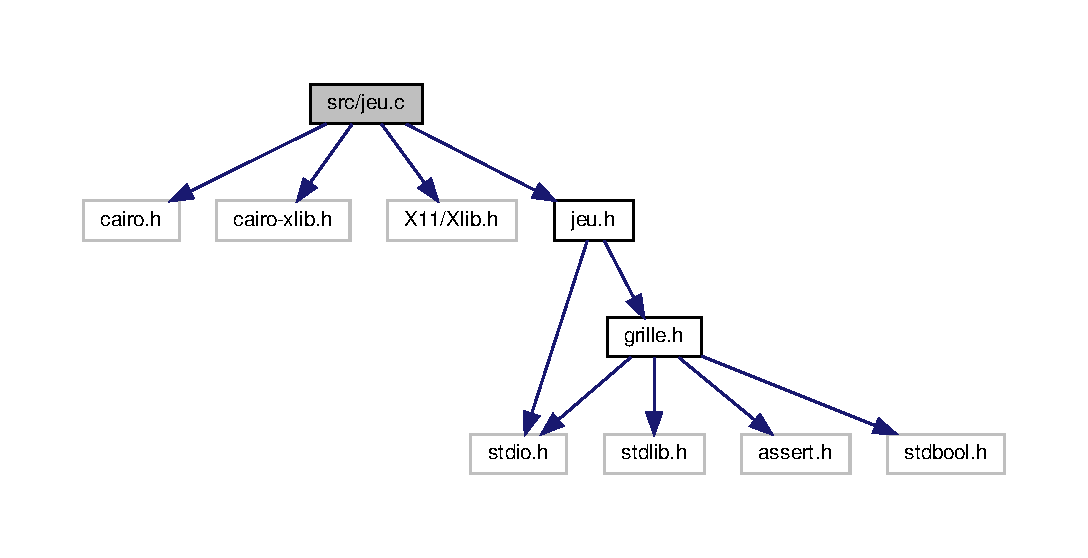
\includegraphics[width=350pt]{jeu_8c__incl}
\end{center}
\end{figure}
\subsection*{Fonctions}
\begin{DoxyCompactItemize}
\item 
int \hyperlink{jeu_8c_acc8422b6280ed6ef09f609683310de92}{compte\+\_\+voisins\+\_\+vivants\+\_\+c} (int i, int j, \hyperlink{structgrille}{grille} g)
\begin{DoxyCompactList}\small\item\em compte le nombre de voisins vivants de la cellule (i,j) avec bords cycliques \end{DoxyCompactList}\item 
int \hyperlink{jeu_8c_a22938221cd19d43dde7cd8fa18e9b3fd}{compte\+\_\+voisins\+\_\+vivants\+\_\+nc} (int i, int j, \hyperlink{structgrille}{grille} g)
\begin{DoxyCompactList}\small\item\em compte le nombre de voisins vivants de la cellule (i,j) sans bords cycliques \end{DoxyCompactList}\item 
void \hyperlink{jeu_8c_a0c11950a46b53162b21b35f8e36757fa}{evolue} (\hyperlink{structgrille}{grille} $\ast$g, \hyperlink{structgrille}{grille} $\ast$gc, int($\ast$compte\+\_\+voisins\+\_\+vivants)(int, int, \hyperlink{structgrille}{grille}), int vieillissement)
\begin{DoxyCompactList}\small\item\em fait evoluer la grille g d\textquotesingle{}un pas de temps \end{DoxyCompactList}\end{DoxyCompactItemize}


\subsection{Description détaillée}
\begin{DoxyAuthor}{Auteur}
D\+AI Yuquan 
\end{DoxyAuthor}


\subsection{Documentation des fonctions}
\mbox{\Hypertarget{jeu_8c_acc8422b6280ed6ef09f609683310de92}\label{jeu_8c_acc8422b6280ed6ef09f609683310de92}} 
\index{jeu.\+c@{jeu.\+c}!compte\+\_\+voisins\+\_\+vivants\+\_\+c@{compte\+\_\+voisins\+\_\+vivants\+\_\+c}}
\index{compte\+\_\+voisins\+\_\+vivants\+\_\+c@{compte\+\_\+voisins\+\_\+vivants\+\_\+c}!jeu.\+c@{jeu.\+c}}
\subsubsection{\texorpdfstring{compte\+\_\+voisins\+\_\+vivants\+\_\+c()}{compte\_voisins\_vivants\_c()}}
{\footnotesize\ttfamily int compte\+\_\+voisins\+\_\+vivants\+\_\+c (\begin{DoxyParamCaption}\item[{int}]{i,  }\item[{int}]{j,  }\item[{\hyperlink{structgrille}{grille}}]{g }\end{DoxyParamCaption})}



compte le nombre de voisins vivants de la cellule (i,j) avec bords cycliques 


\begin{DoxyParams}{Paramètres}
{\em i} & position i \\
\hline
{\em j} & position j \\
\hline
{\em g} & grille \\
\hline
\end{DoxyParams}
\begin{DoxyReturn}{Renvoie}
v le nombre de voisins vivants de la cellule (i, j) 
\end{DoxyReturn}
\mbox{\Hypertarget{jeu_8c_a22938221cd19d43dde7cd8fa18e9b3fd}\label{jeu_8c_a22938221cd19d43dde7cd8fa18e9b3fd}} 
\index{jeu.\+c@{jeu.\+c}!compte\+\_\+voisins\+\_\+vivants\+\_\+nc@{compte\+\_\+voisins\+\_\+vivants\+\_\+nc}}
\index{compte\+\_\+voisins\+\_\+vivants\+\_\+nc@{compte\+\_\+voisins\+\_\+vivants\+\_\+nc}!jeu.\+c@{jeu.\+c}}
\subsubsection{\texorpdfstring{compte\+\_\+voisins\+\_\+vivants\+\_\+nc()}{compte\_voisins\_vivants\_nc()}}
{\footnotesize\ttfamily int compte\+\_\+voisins\+\_\+vivants\+\_\+nc (\begin{DoxyParamCaption}\item[{int}]{i,  }\item[{int}]{j,  }\item[{\hyperlink{structgrille}{grille}}]{g }\end{DoxyParamCaption})}



compte le nombre de voisins vivants de la cellule (i,j) sans bords cycliques 


\begin{DoxyParams}{Paramètres}
{\em i} & position i \\
\hline
{\em j} & position j \\
\hline
{\em g} & grille \\
\hline
\end{DoxyParams}
\begin{DoxyReturn}{Renvoie}
v le nombre de voisins vivants de la cellule (i, j) 
\end{DoxyReturn}
\mbox{\Hypertarget{jeu_8c_a0c11950a46b53162b21b35f8e36757fa}\label{jeu_8c_a0c11950a46b53162b21b35f8e36757fa}} 
\index{jeu.\+c@{jeu.\+c}!evolue@{evolue}}
\index{evolue@{evolue}!jeu.\+c@{jeu.\+c}}
\subsubsection{\texorpdfstring{evolue()}{evolue()}}
{\footnotesize\ttfamily void evolue (\begin{DoxyParamCaption}\item[{\hyperlink{structgrille}{grille} $\ast$}]{g,  }\item[{\hyperlink{structgrille}{grille} $\ast$}]{gc,  }\item[{int($\ast$)(int, int, \hyperlink{structgrille}{grille})}]{compte\+\_\+voisins\+\_\+vivants,  }\item[{int}]{vieillissement }\end{DoxyParamCaption})}



fait evoluer la grille g d\textquotesingle{}un pas de temps 


\begin{DoxyParams}{Paramètres}
{\em g} & grille \\
\hline
{\em gc} & grille \\
\hline
{\em ($\ast$compte\+\_\+voisins\+\_\+vivants)(int,int,grille)} & pointeur vers une fonction \\
\hline
{\em vieillissement} & une cellule meurt de viellesse quand son âge dépasse 8 pas de temps \\
\hline
\end{DoxyParams}

\hypertarget{jeu_8h}{}\section{Référence du fichier jeu.\+h}
\label{jeu_8h}\index{jeu.\+h@{jeu.\+h}}


Fichier entête du code source \hyperlink{jeu_8c}{jeu.\+c}.  


{\ttfamily \#include \char`\"{}grille.\+h\char`\"{}}\newline
{\ttfamily \#include $<$stdio.\+h$>$}\newline
Graphe des dépendances par inclusion de jeu.\+h\+:
% FIG 0
Ce graphe montre quels fichiers incluent directement ou indirectement ce fichier \+:
% FIG 1
\subsection*{Macros}
\begin{DoxyCompactItemize}
\item 
\mbox{\Hypertarget{jeu_8h_ac6afabdc09a49a433ee19d8a9486056d}\label{jeu_8h_ac6afabdc09a49a433ee19d8a9486056d}} 
\#define {\bfseries min}(a,  b)~((a) $<$ (b) ? (a) \+: (b))
\item 
\mbox{\Hypertarget{jeu_8h_affe776513b24d84b39af8ab0930fef7f}\label{jeu_8h_affe776513b24d84b39af8ab0930fef7f}} 
\#define {\bfseries max}(a,  b)~((a) $>$ (b) ? (a) \+: (b))
\end{DoxyCompactItemize}
\subsection*{Fonctions}
\begin{DoxyCompactItemize}
\item 
int \hyperlink{jeu_8h_acc8422b6280ed6ef09f609683310de92}{compte\+\_\+voisins\+\_\+vivants\+\_\+c} (int i, int j, \hyperlink{structgrille}{grille} g)
\begin{DoxyCompactList}\small\item\em compte le nombre de voisins vivants de la cellule (i,j) avec bords cycliques \end{DoxyCompactList}\item 
int \hyperlink{jeu_8h_a22938221cd19d43dde7cd8fa18e9b3fd}{compte\+\_\+voisins\+\_\+vivants\+\_\+nc} (int i, int j, \hyperlink{structgrille}{grille} g)
\begin{DoxyCompactList}\small\item\em compte le nombre de voisins vivants de la cellule (i,j) sans bords cycliques \end{DoxyCompactList}\item 
void \hyperlink{jeu_8h_a0c11950a46b53162b21b35f8e36757fa}{evolue} (\hyperlink{structgrille}{grille} $\ast$g, \hyperlink{structgrille}{grille} $\ast$gc, int($\ast$compte\+\_\+voisins\+\_\+vivants)(int, int, \hyperlink{structgrille}{grille}), int vieillissement)
\begin{DoxyCompactList}\small\item\em fait evoluer la grille g d\textquotesingle{}un pas de temps \end{DoxyCompactList}\end{DoxyCompactItemize}


\subsection{Description détaillée}
Fichier entête du code source \hyperlink{jeu_8c}{jeu.\+c}. 

\begin{DoxyAuthor}{Auteur}
D\+AI Yuquan 
\end{DoxyAuthor}


\subsection{Documentation des fonctions}
\mbox{\Hypertarget{jeu_8h_acc8422b6280ed6ef09f609683310de92}\label{jeu_8h_acc8422b6280ed6ef09f609683310de92}} 
\index{jeu.\+h@{jeu.\+h}!compte\+\_\+voisins\+\_\+vivants\+\_\+c@{compte\+\_\+voisins\+\_\+vivants\+\_\+c}}
\index{compte\+\_\+voisins\+\_\+vivants\+\_\+c@{compte\+\_\+voisins\+\_\+vivants\+\_\+c}!jeu.\+h@{jeu.\+h}}
\subsubsection{\texorpdfstring{compte\+\_\+voisins\+\_\+vivants\+\_\+c()}{compte\_voisins\_vivants\_c()}}
{\footnotesize\ttfamily int compte\+\_\+voisins\+\_\+vivants\+\_\+c (\begin{DoxyParamCaption}\item[{int}]{i,  }\item[{int}]{j,  }\item[{\hyperlink{structgrille}{grille}}]{g }\end{DoxyParamCaption})}



compte le nombre de voisins vivants de la cellule (i,j) avec bords cycliques 


\begin{DoxyParams}{Paramètres}
{\em i} & position i \\
\hline
{\em j} & position j \\
\hline
{\em g} & grille \\
\hline
\end{DoxyParams}
\begin{DoxyReturn}{Renvoie}
v le nombre de voisins vivants de la cellule (i, j) 
\end{DoxyReturn}
\mbox{\Hypertarget{jeu_8h_a22938221cd19d43dde7cd8fa18e9b3fd}\label{jeu_8h_a22938221cd19d43dde7cd8fa18e9b3fd}} 
\index{jeu.\+h@{jeu.\+h}!compte\+\_\+voisins\+\_\+vivants\+\_\+nc@{compte\+\_\+voisins\+\_\+vivants\+\_\+nc}}
\index{compte\+\_\+voisins\+\_\+vivants\+\_\+nc@{compte\+\_\+voisins\+\_\+vivants\+\_\+nc}!jeu.\+h@{jeu.\+h}}
\subsubsection{\texorpdfstring{compte\+\_\+voisins\+\_\+vivants\+\_\+nc()}{compte\_voisins\_vivants\_nc()}}
{\footnotesize\ttfamily int compte\+\_\+voisins\+\_\+vivants\+\_\+nc (\begin{DoxyParamCaption}\item[{int}]{i,  }\item[{int}]{j,  }\item[{\hyperlink{structgrille}{grille}}]{g }\end{DoxyParamCaption})}



compte le nombre de voisins vivants de la cellule (i,j) sans bords cycliques 


\begin{DoxyParams}{Paramètres}
{\em i} & position i \\
\hline
{\em j} & position j \\
\hline
{\em g} & grille \\
\hline
\end{DoxyParams}
\begin{DoxyReturn}{Renvoie}
v le nombre de voisins vivants de la cellule (i, j) 
\end{DoxyReturn}
\mbox{\Hypertarget{jeu_8h_a0c11950a46b53162b21b35f8e36757fa}\label{jeu_8h_a0c11950a46b53162b21b35f8e36757fa}} 
\index{jeu.\+h@{jeu.\+h}!evolue@{evolue}}
\index{evolue@{evolue}!jeu.\+h@{jeu.\+h}}
\subsubsection{\texorpdfstring{evolue()}{evolue()}}
{\footnotesize\ttfamily void evolue (\begin{DoxyParamCaption}\item[{\hyperlink{structgrille}{grille} $\ast$}]{g,  }\item[{\hyperlink{structgrille}{grille} $\ast$}]{gc,  }\item[{int($\ast$)(int, int, \hyperlink{structgrille}{grille})}]{compte\+\_\+voisins\+\_\+vivants,  }\item[{int}]{vieillissement }\end{DoxyParamCaption})}



fait evoluer la grille g d\textquotesingle{}un pas de temps 


\begin{DoxyParams}{Paramètres}
{\em g} & grille \\
\hline
{\em gc} & grille \\
\hline
{\em ($\ast$compte\+\_\+voisins\+\_\+vivants)(int,int,grille)} & pointeur vers une fonction \\
\hline
{\em vieillissement} & une cellule meurt de viellesse quand son âge dépasse 8 pas de temps \\
\hline
\end{DoxyParams}

\hypertarget{main_8c}{}\section{Référence du fichier main.\+c}
\label{main_8c}\index{main.\+c@{main.\+c}}
{\ttfamily \#include $<$stdio.\+h$>$}\newline
{\ttfamily \#include $<$string.\+h$>$}\newline
{\ttfamily \#include $<$unistd.\+h$>$}\newline
{\ttfamily \#include \char`\"{}grille.\+h\char`\"{}}\newline
{\ttfamily \#include \char`\"{}io.\+h\char`\"{}}\newline
{\ttfamily \#include \char`\"{}jeu.\+h\char`\"{}}\newline
Graphe des dépendances par inclusion de main.\+c\+:
% FIG 0
\subsection*{Fonctions}
\begin{DoxyCompactItemize}
\item 
int \hyperlink{main_8c_a3c04138a5bfe5d72780bb7e82a18e627}{main} (int argc, char $\ast$$\ast$argv)
\begin{DoxyCompactList}\small\item\em execute le jeu \end{DoxyCompactList}\end{DoxyCompactItemize}


\subsection{Description détaillée}
\begin{DoxyAuthor}{Auteur}
D\+AI Yuquan 
\end{DoxyAuthor}


\subsection{Documentation des fonctions}
\mbox{\Hypertarget{main_8c_a3c04138a5bfe5d72780bb7e82a18e627}\label{main_8c_a3c04138a5bfe5d72780bb7e82a18e627}} 
\index{main.\+c@{main.\+c}!main@{main}}
\index{main@{main}!main.\+c@{main.\+c}}
\subsubsection{\texorpdfstring{main()}{main()}}
{\footnotesize\ttfamily int main (\begin{DoxyParamCaption}\item[{int}]{argc,  }\item[{char $\ast$$\ast$}]{argv }\end{DoxyParamCaption})}



execute le jeu 


\begin{DoxyParams}{Paramètres}
{\em argv} & repertoire du fichier avec la grille \\
\hline
\end{DoxyParams}
\begin{DoxyReturn}{Renvoie}
0 si l\textquotesingle{}utilisateur a appuye sur \textquotesingle{}q\textquotesingle{} 
\end{DoxyReturn}

%--- End generated contents ---

% Index
\backmatter
\newpage
\phantomsection
\clearemptydoublepage
\addcontentsline{toc}{chapter}{Index}
\printindex

\end{document}
